
\begin{enumerate}
    \item A block of weight 100 N is suspended by copper and steel wires of same cross sectional area 0.5 cm\(^2\) and, length \(\sqrt{3}\) m and 1 m, respectively. Their other ends are fixed on a ceiling as shown in figure. The angles subtended by copper and steel wires with ceiling are 30\(^{\circ}\) and 60\(^{\circ}\), respectively. If elongation in copper wire is (\(\Delta l_c\)) and elongation in steel wire is (\(\Delta l_s\)), then the ratio \(\frac{\Delta l_c}{\Delta l_s}\) is \_\_\_. 
    [Young’s modulus for copper and steel are \(1\times10^{11}\) N/m\(^2\) and \(2\times10^{11}\) N/m\(^2\), respectively.]

    \centering
    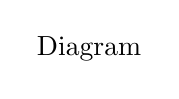
\begin{tikzpicture}
        % This is just a placeholder for the actual diagram.
        \node {Diagram};
    \end{tikzpicture}
\end{enumerate}
